\documentclass[a4paper]{article}

%% Language and font encodings
\usepackage[french]{babel}
\usepackage[utf8x]{inputenc}
\usepackage[T1]{fontenc}
\usepackage{wrapfig}

%% Sets page size and margins
\usepackage[a4paper,top=3cm,bottom=2cm,left=3cm,right=3cm,marginparwidth=1.75cm]{geometry}

%% Useful packages
\usepackage{amsmath}
\usepackage{graphicx}
\usepackage[colorinlistoftodos]{todonotes}
\usepackage[colorlinks=true, allcolors=blue, breaklinks=true]{hyperref}

\newcommand{\guill}[1]{\og{}#1\fg{}}

\title{Attaques par "canal auxiliaire"}
\author{Maude Pupin et Julien Narboux}

\begin{document}
\maketitle

\begin{abstract}
Description d'une activité d'informatique débranchée sur le thème des attaques par \guill{canal auxiliaire}.
Cette activité a été préparée lors de l’École sur la \href{https://www.societe-informatique-de-france.fr/ecole-mediation-scientifique-en-informatique/}{médiation informatique de la SIF} en Juin 2018.  L'idée de l'activité a été proposée par Pascal Lafourcade avec la participation de David Cachera et Cécile Pierrot.
\end{abstract}

\section{Matériel}

\begin{itemize}
\item Le dessin d'un clavier numérique (voir dernière page).
\item Éventuellement un objet pour indiquer qu'un code est faux (lampe rouge ou morceau de papier)  
\item Un ordinateur pour la dernière partie en branchée.
\end{itemize}

\section{Déroulé de l'activité}

\subsection{Introduction}
On commence par la question: \guill{Quelle est la différence entre un ordinateur et un humain ?}
On attend la réponse: \guill{ordinateur rapide mais bête, humain intelligent mais lent}.

\guill{Bonjour, aujourd'hui vous allez ouvrir un coffre fort.
Pour la première étape, je vais remplacer le coffre fort en exécutant un programme pour vérifier si le code est correct.
Mais comme je suis un humain, je ne suis pas rapide alors allez lentement !
C'est une coffre fort mal conçu, vous allez donc peut-être pouvoir trouver la combinaison rapidement. Essayez !}

\subsection{Exploration du premier coffre}

\begin{wrapfigure}{R}{0.3\textwidth}
\centering
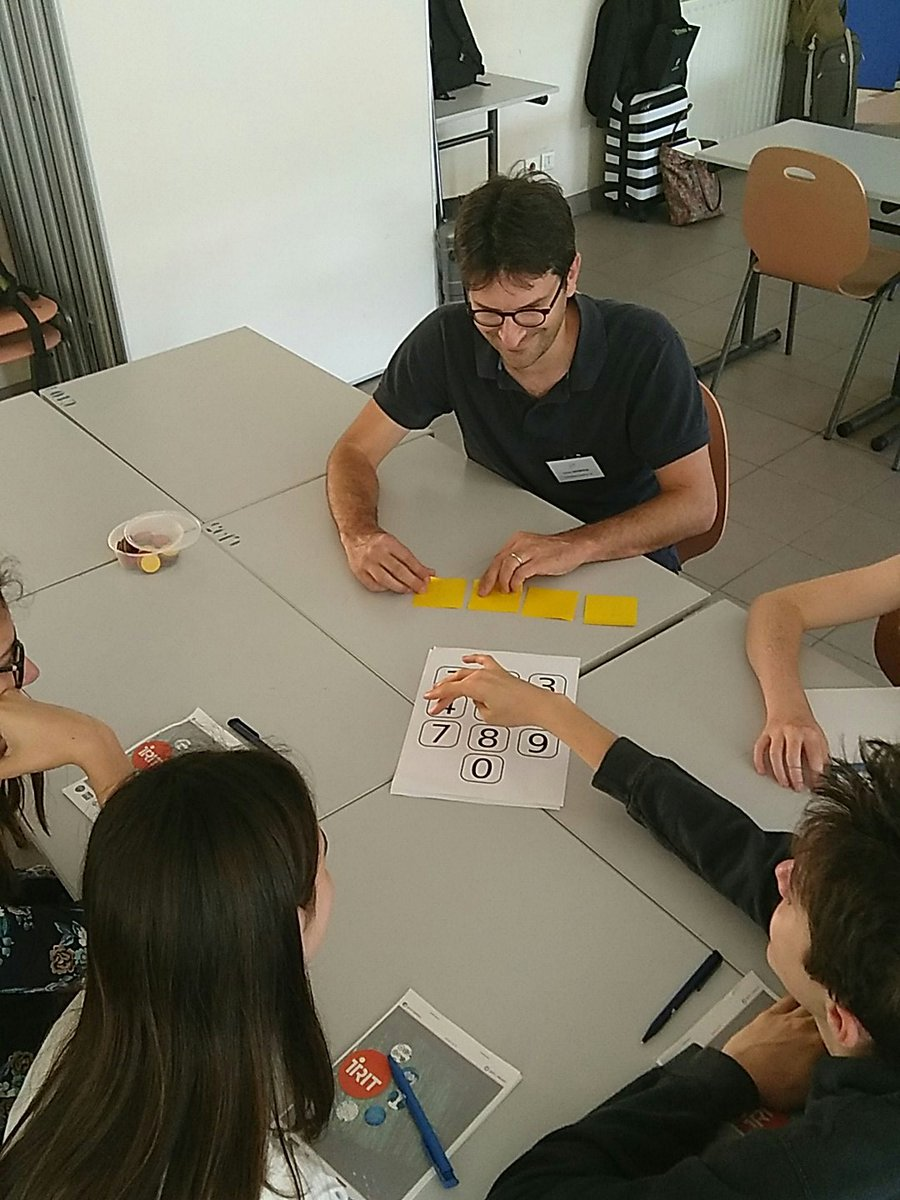
\includegraphics[width=0.25\textwidth]{digicode-ecole-sif.jpg}
\end{wrapfigure}


On choisit un code à quatre chiffres, on laisse les participants appuyer sur notre clavier en papier, \textbf{dès qu'un chiffre} est faux on l'indique à l'aide d'un objet ou en faisant un bruit\footnote{La question se pose de savoir quel genre de digicode on simule, est-ce que l'on repart à zéro dès qu'un chiffre est faux ou est-ce qu'il faut un temps d'attente entre deux tentatives ?}.

D'expérience avec des élèves de secondes, les participants vont vite commencer à explorer plusieurs code et trouver la solution.


\subsection{Analyse de l'exploration du premier coffre}

Question: \guill{Pourquoi ce coffre est mal conçu ?}.
Réponse attendue: \guill{Parce qu'il répond dès qu'un chiffre est faux sans attendre les quatre}.

On peut continuer en demandant combien d'essais au maximum il faudra réaliser pour trouver le code.

Réponse attendue: En 4*10 essais on sera sûr d'avoir trouvé le code.

À mettre en opposition avec le nombre de propositions à faire si on n'avait aucune indication pendant la saisie, ce qui correspond au nombre de codes différents à quatre chiffres. Il faut aussi leur demander combien il y en a.
Pour aider on peut reformuler, \guill{combien y a-t-il de possibilités pour le premier chiffre, etc.}
Puis, s'ils ne trouvent toujours pas, on peut demander: \guill{Jusqu'à quel nombre peut-on compter avec 4 chiffres ?}


\subsection{Exploration du deuxième coffre}

\begin{wrapfigure}{R}{0.3\textwidth}
\centering
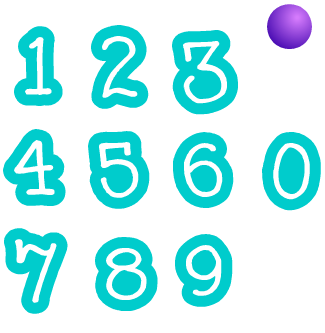
\includegraphics[width=0.25\textwidth]{scratch-digicode-screen.png}
\end{wrapfigure}

\guill{Ok, c'était facile ! Maintenant, je vais vous proposer un deuxième coffre pas très bien conçu non plus. À vous de trouver la combinaison.}

\begin{wrapfigure}{R}{0.5\textwidth}
\centering
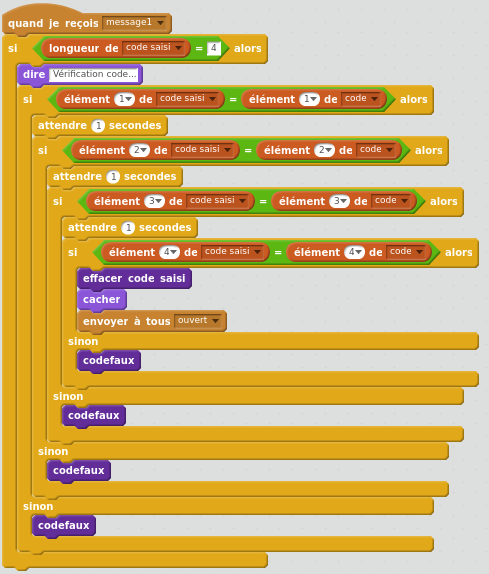
\includegraphics[width=0.45\textwidth]{scratch-digicode.png}
\end{wrapfigure}

Ce coffre est matérialisé par un programme Scratch disponible 
\href{https://scratch.mit.edu/projects/228338538/#player}{ici}.

On ne montre pas le programme aux participants, le coffre doit rester une boite noire. Le code secret est la date de naissance d'Ada Lovelace, ça permet éventuellement de faire une parenthèse en posant la question \guill{Qui était le premier programmeur ?}.

Si les participants ne trouvent pas la faille, on peut donner une indication:
\guill{Est-ce que tu as un chronomètre sur toi ?}

\subsection{Explications}

\guill{Ici notre exemple est simplifié pour que l'on puisse deviner le code en chronométrant grossièrement.
Mais dans la réalité ce genre de failles ont déjà été exploitées: on peut exploiter par exemple le temps de réponse d'un algorithme qui décide si un code est correct ou non pour obtenir de l'information sur ce code. On peut aussi exploiter la consommation électrique, toutes les instructions exécutées par une carte à puce ne consomment pas forcement la même quantité d'énergie.
Depuis que ce genre de failles est connu, on essaie de concevoir des puces qui consomment tout le temps la même quantité d'énergie. Pour plus d'informations voir l'article d'Hélène Le Bouder \href{https://interstices.info/jcms/p_91127/des-attaques-informatiques-utilisant-la-physique}{Des attaques informatiques utilisant la physique}
}

\section{Retours d'expériences}

On a testé avec une classe de seconde uniquement en débranché, sans l'application Scratch. Il fallait environ 15 minutes pour faire l'activité (sans le deuxième coffre).

On pourrait améliorer l'activité en essayant de ne pas utiliser d'ordinateur. Voici deux pistes non explorées:
\begin{enumerate}
\item Remplacer le programme Scratch par un objet avec un vrai clavier et une LED pilotés par un Arduino.
\item Présenter l'activité sous forme d'un tour de magie:
 \begin{itemize}
  \item Les participants choisissent un code à trois chiffres.
  \item Quand le magicien essaie un code, ils doivent exécuter à la main un petit programme.
Par exemple, le programme pourrait consister à dessiner des choses au moyens de feutres, le magicien ne voit pas les dessins mais uniquement les feutres utilisés, suivant les feutres utilisés on en déduirait le nombre de chiffres corrects.
 \end{itemize} 
\end{enumerate}

%On pourrait aussi prolonger l'activité en essayant d'expliquer le pipeline d'un microprocesseur à l'aide de jouets: une mini machine à laver, une mini-machine à sécher le linge vs une machine lavante - séchante.

%Quelques productions et/ou retours des participants, si disponibles
% Ils sont chez moi, je les scanne quand j'ai le temps.

\section{Liens:}
\begin{itemize}
\item \href{https://scratch.mit.edu/projects/228338538/#player}{Programme Scratch}
\item \href{https://fr.wikipedia.org/wiki/Attaque_par_canal_auxiliaire}{Wikipedia - Attaque par canal auxiliaire}
\item \href{https://interstices.info/jcms/p_91127/des-attaques-informatiques-utilisant-la-physique}{Article dans Interstices de Hélène Le Bouder}
\end{itemize}

%\bibliographystyle{alpha}
%\bibliography{sample}

\newpage
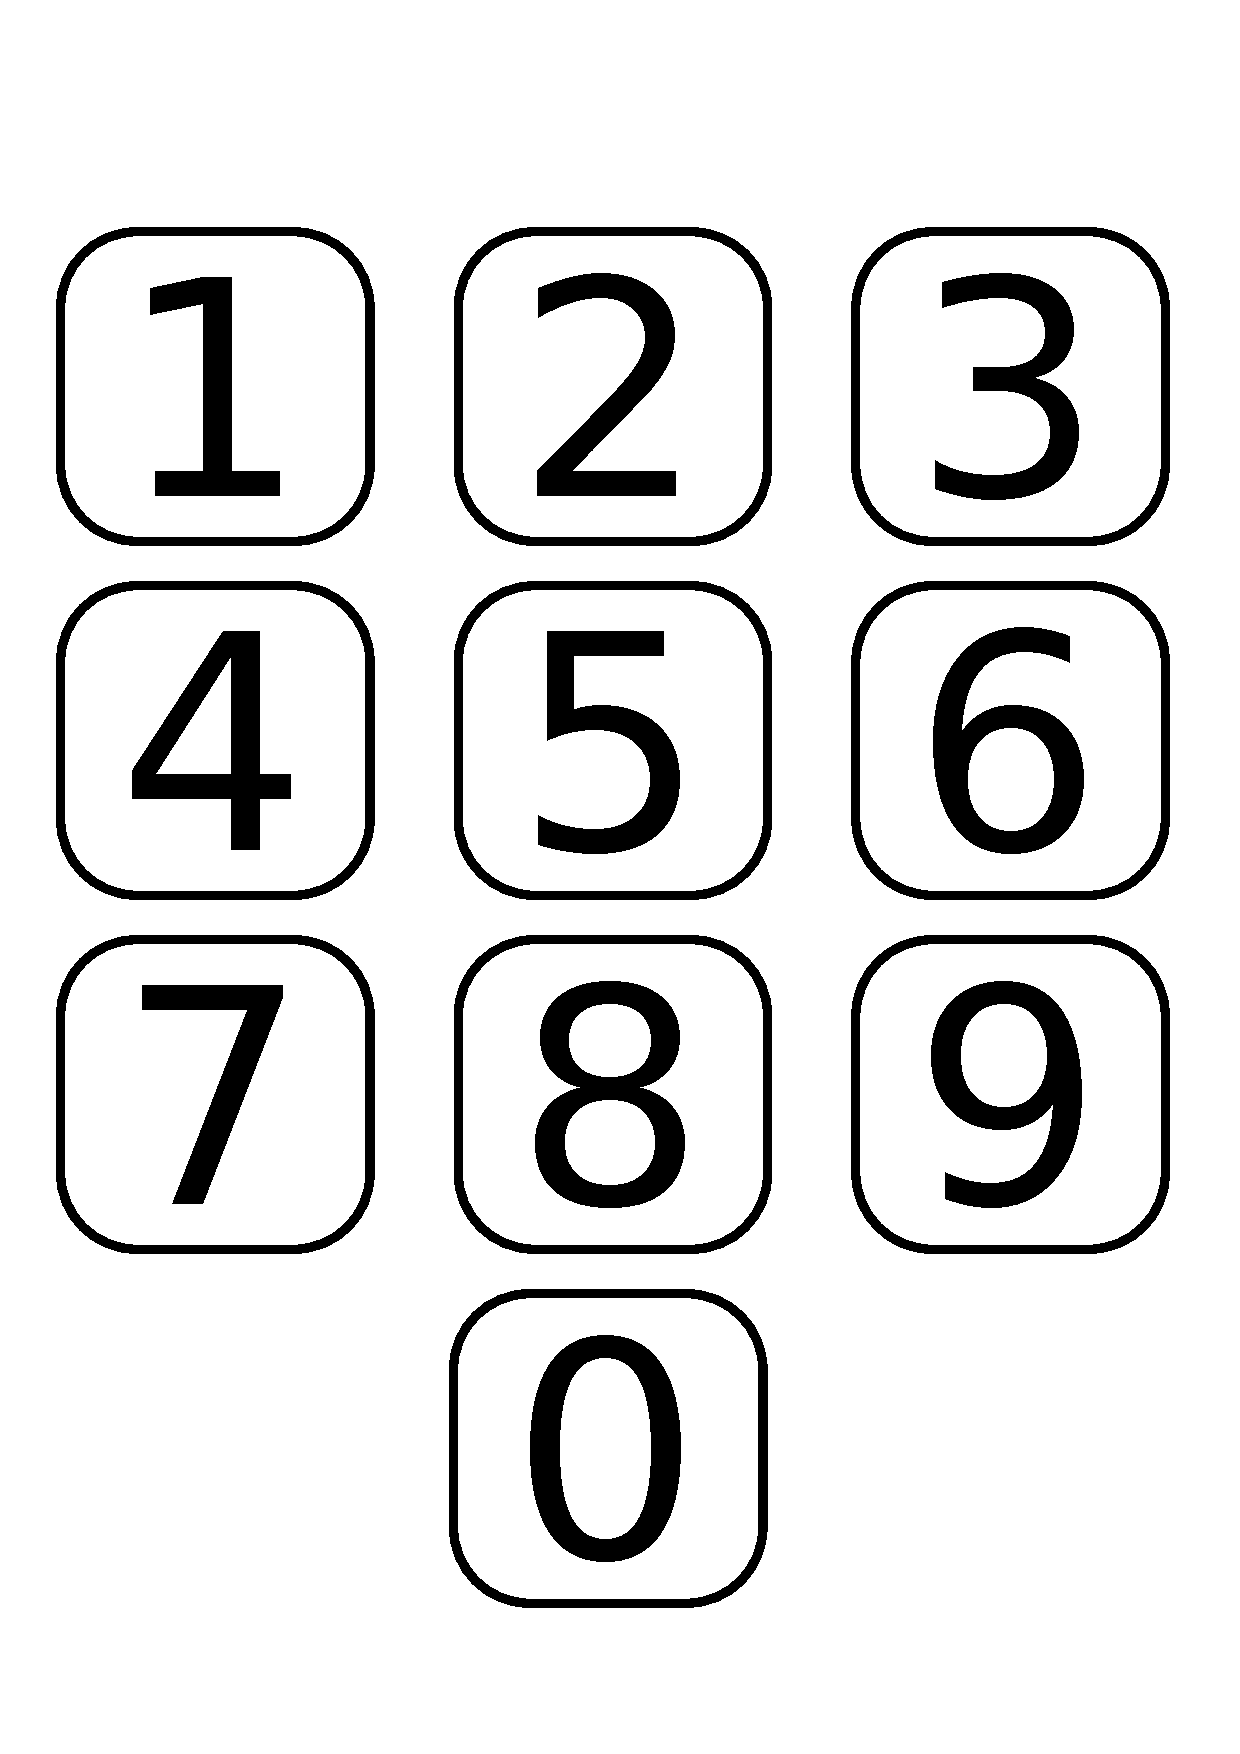
\includegraphics[width=\textwidth]{digicode.pdf}


\end{document}